\documentclass[10pt]{beamer}
\usepackage[T1]{fontenc}
\usepackage{xeCJK}
\usepackage{listings}
\usepackage{xcolor}
\usepackage[ruled,linesnumbered]{algorithm2e}

\definecolor{mygreen}{rgb}{0,0.6,0}
\definecolor{mygray}{rgb}{0.5,0.5,0.5}
\definecolor{mymauve}{rgb}{0.58,0,0.82}
\lstset{ %
	backgroundcolor=\color{white},   % choose the background color
	basicstyle=\footnotesize\rmfamily,     % size of fonts used for the code
	columns=fullflexible,
	breaklines=true,                 % automatic line breaking only at whitespace
	captionpos=b,                    % sets the caption-position to bottom
	tabsize=4,
	commentstyle=\color{mygreen},    % comment style
	escapeinside={\%*}{*)},          % if you want to add LaTeX within your code
	keywordstyle=\color{blue},       % keyword style
	stringstyle=\color{mymauve}\ttfamily,     % string literal style
	numbers=left, 
%	frame=single,
	rulesepcolor=\color{red!20!green!20!blue!20},
  % identifierstyle=\color{red},
  language=c
}

\usetheme{Madrid}

\title{Hello World}
\subtitle[short subtitle]{long subtitle}
\author[dxy]{Xiangyun Ding}
\institute{Tsinghua University}
\date{March 1, 2020}  % \date{\today}

% \small \tiny \large \huge 以及大写的

\AtBeginSection[]
{
	\begin{frame}<beamer>
	  \frametitle{\textbf{目录}}
	  \tableofcontents[currentsection]
  \end{frame}
}

\begin{document}

\frame{\titlepage}

\section[目录]{}   %目录
\begin{frame}{目录}
\tableofcontents
\end{frame}

\section{section1}

\begin{frame}{A sample slide}

  \href{http://v.youku.com/}{一个超链接} 

A displayed formula:
\[
  \int_{-\infty}^\infty e^{-x^2}dx = \sqrt{\pi}
\]
An itemized list:

\begin{itemize}
  \item itemized item 1,你好
  \item itemized item 2
\end{itemize}
\begin{enumerate}
  \item The first item
  \item The second item
\end{enumerate}

\end{frame}

\begin{frame}

\begin{theorem}{1.1}
  In a right triangle, \small{the square of hypotenuse equals
  the sum of squares of two} other sides.
\end{theorem}

\begin{block}{123}
  hello
\end{block}

\begin{description}
  \item[First Item] Description of first item
  \vspace{0.5cm}  %空一行 
  \item[Second Item] Description of second item
\end{description}

\begin{columns}
  \column{.50\textwidth}
  First column text and/or code
  \column{.50\textwidth}
  Second column text and/or code
\end{columns}

\end{frame}

\section{section2}

\begin{frame}{fff}
  \begin{table}
    \centering
    \caption{table decription}
    \label{t_sim}
    \begin{tabular}{|l|l|}
    \hline
    \textbf{Key} & \textbf{Value} \\
    \hline
    $x$ & description of x \\
    $y$ & description of y \\
    $y$ & description of z \\
    \hline
    \end{tabular}
    \end{table}

    \begin{table}[tb]
      \centering
      \caption{Caption here\label{tab:tablename}}
      \begin{tabular}{l|cc}
      \hline
      \textbf{column 1} & \textbf{column 2} & \textbf{column 3} \\ \hline
      Hello & Beamer & NAN \\ \hline
      $\alpha+\beta$ & $\gamma+\eta$ & 34\% \\ \hline
      \end{tabular}
      \end{table}

\end{frame}

\begin{frame}

  \begin{figure}[tb]
    \label{fig:figure1}
    \centering
    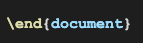
\includegraphics[width=0.5\textwidth]{t1.png}
    \caption{Caption here}
  \end{figure}

\end{frame}

\begin{frame}{代码}

  \lstinputlisting[lastline=30,
language=Python,
frame=single,
label=python]
{temp.py}

\end{frame}

\begin{frame}{算法}
  \begin{algorithm}[H]
    \caption{HOSVD}
    \small 
    \KwIn{HOSVD($\mathcal{X},R_{1},R_{2}.....R_{N}$) }
    \KwOut{ $\mathcal{G},A_{(1)},A_{(2)}......A_{(N)} $ }
    
    \For{$k=1$ to $N$ }
    {
      $A_{(n)}\leftarrow R_{n}$left singular matrix of $X_{(n)}$
    }
    $\mathcal{G}=\leftarrow \mathcal{X} \times A_{(1)}^{T} \times A_{(2)}^{T}...... \times A_{(N)}^{T}$\\
    \Return $\mathcal{G},A_{(1)},A_{(2)}......A_{(N)} $
  \end{algorithm}
  \end{frame}

\section{section3}
\begin{frame}{研究方法与数据集特征}
  \begin{itemize}
    \item<1-> First point, shown on all slides.
    \item<2-> Second point, shown on slide 2 and later.
    \item<3-> Third point, also shown on slide 2 and later.
    \item<4-> Fourth point, shown on slide 3.
  \end{itemize}
\end{frame}

\begin{frame}
  \hspace{3cm}
  \Huge{Questions?}
\end{frame}

\end{document}